\section{FEM Validation With Sample Path Method}

In this section, the solutions to the FPE obtained with the FEM are reproduced using an alternate approach. Instead of solving the FPE, the underlying stochastic differential equations are solved numerically. The validation method presented in this section can be used with the autoparametric and the wave systems, but results have been computed only for the autoparametric oscillator. The method presented was inspired by the heterogeneous multiscale method, as applied to stochastic differential equations \citep{e05:_analy}.

To begin, recall that unperturbed dynamics are governed by a Hamiltonian
\[
\dot z = \bar \nabla K, \quad z_0 \in \Real^4.
\]
After a canonical transformation, the dynamics of $z$ can be separated so that the fast dynamics are restricted to being in a 2-D plane. For the autoparametric oscillator, recalling Equation \eqref{E:vector-int}, the fast dynamics were given by
\begin{align*}
\dot u_1 &= - u_1 u_2, & \dot u_2 &= \frac12 (3 u_1^2 + u_2^2 - I).
\end{align*}
For the surface gravity wave model, similar 2-D fast dynamics are described by Equation \eqref{e:sgwaves fast planar}. These dynamics are obtained after time averaging and they are perturbed by higher order noise and damping effects. $X_t = (u_1,u_2)$ will be used as the fast variables and $Y_t = (K,I)$ will be the slow variables. Note that because $u_1, u_2$ and $K$ are constrained by Equation \eqref{E:AvgH}, it should be possible to have only one of the variables from the $(u_1,u_2)$ pair as the fast variable, but computationally it seems easier to use Equation \eqref{E:vector-int} than Equation \eqref{E:AvgH}. The general form of the fast equations is
\[
d X_t = \epsilon^{-2} f(X_t,Y_t) dt
\]
After time-averaging, the slow dynamics are given by
\begin{equation}
d \Tave[Y_t] = \epsilon^{-1} \Tave[F^2](X_t,Y_t) dt + \epsilon^{-2} \Tave[G](X_t,Y_t) dt.
\end{equation}
It is important to understand why the dynamics of the slow variables are time averaged. Prior to time averaging, the equation for $Y_t$ contains a term of order $\epsilon^{-2}$, therefore the dynamical timescales of the fast and slow equations are not separated. It should be possible to perform $\Tave$-averaging numerically, but for simplicity, here time averaged quantities are considered straightaway.
The averaged equation is
\begin{equation}
\label{e:averaged}
d\Aave[\Tave[Y_t]] = \Aave[\Tave[m]](Y_t) dt + \Aave[\Tave[\sigma]](Y_t) dt
\end{equation}
with $m$ defined in Equation \eqref{E:drift2} and $\sigma$ will be derived from \eqref{E:diffusion2}. Conceptually, $\Aave$-averaging represents averages over Hamiltonian orbits.

Having described the two timescale nature the equations to be solved, now the numerical procedure is setup. Since the fast dynamics are deterministic, the equivalent of what is called the \emph{microsolver} in the HMM can be implemented using widely available numerical ODE solvers. The microsolver serves to generate paths over which to calculate the averaged coefficients, symbolically
\[
\Aave[f](y) = \frac{1}{T(y)} \int_0^{T(y)} f(X_t, y) dt.
\]
For simplicity analytic results of Chapter \ref{c:autoparametric} are used for $T(y)$, but in principle this quantity could be discovered with the microsolver. Note that in \citet{e05:_analy} the case where the fast equations are stochastic is treated; this can make the choice of an optimal time-span for the microsolver more difficult. Referring to terminology used in the HMM context, an \emph{estimator} is used to approximate the averaging operator. The estimator resembles numerical integration formulas:
\[
\frac{1}{T(y)} \sum_{i=1}^N f(u(t_i),y) \Delta t_i.
\]
Thus estimated values for $\Aave[\Tave[m]]$ and $\Aave[\Tave[\sigma \sigma^T]]$ are obtained. Let us denote these estimates by $\tilde{\mathfrak b}$ and $\tilde{\mathfrak a}$ respectively. Because the fast equations are deterministic, the computations performed by the microsolver and estimator for the problems considered in this thesis are rather simple. Nonetheless, they make it possible to validate the results obtained analytically for the autoparametric oscillator and the results obtained with numerical quadrature for the surface gravity waves system. Comparisons between the analytically obtained drift and diffusion coefficients and their estimated values show good agreement (typically differences smaller than $10^{-8}$.)

Whereas averaging provides the diffusion matrix $\mathfrak{a} = \Aave[\Tave[\sigma \sigma^T]]$, to produce sample paths, $\sigma$ is needed. Cholesky decomposition is used to make this connection. Symbolically, let's use the notation
\[
\tilde{\mathfrak a} = \tilde \sigma \tilde \sigma^T.
\]
The key point is that the variance of $\tilde{\mathfrak a}$ is reproduced when $\tilde \sigma^T$ multiplies a Wiener process \citep{law82:_simul}.

In the HMM, the slow equations are approximated numerically with the \emph{macrosolver}. For numerical solutions to System \eqref{e:averaged}, a stochastic ODE solver is used. The simplest of these is the Euler-Maruyama first order scheme \citep{kloeden99:_numer_solut_stoch_differ_equat}:
\[
Y_{n+1} = Y_n + \tilde{\mathfrak b}_n \Delta t + \tilde \sigma_n \Xi_{n+1} \sqrt{\Delta t}
\]
where $\Xi_n$ are normally distributed random numbers with mean zero and variance one. This completes the description of the numerical method used to generate stochastic samples in a multiscale context. An analysis of the convergence properties and efficiency of the scheme presented here has not been performed.

In order to validate the solutions obtained by the FEM multiple sample paths must be produced. This can be done systematically with the following procedure. First, initial conditions must be generated so as to reproduce a uniform distribution across the entire $K-I$ domain. First a FEM triangulation is produced and the area of each element is calculated. The initial conditions of the samples are set at the center of each element, and the number of samples in each element is proportional to each element's area. Such a placement scheme is automated by dividing the unit interval into segments with length proportional to each element's area. A uniform random number generator is then used to draw numbers in the unit interval and the number of samples placed at the center of each element is determined by the uniform random number generator. Thus larger elements end up with more samples and smaller elements with fewer.

At each time-step of the macrosolver, the microsolver is initialized with conditions consistent with the state of the macrosolver. The microsolver is then simulated for the time-span of one period so as to compute the values of $\tilde{\mathfrak b}$ and $\tilde{\mathfrak a}$. In order to impose reflective boundary conditions, at each step of the macrosolver a check is made to determine if the sample has gone outside the domain. If it has, the sample is returned to its last location inside the domain, but the time-step is still increased by one. This approach ensure that the reflective boundary condition does not lead to infinite simulation times.

% FIXME Provide pseudo-code of the function macrosolver_ic here.

All the samples are simulated for an equal number of time-steps of the macrosolver. The number of samples in each element is then counted and the value of each node is set by taking the average of the number of samples of all the elements that contain that node.

% FIXME The average should, perhaps, be weighed by the element areas.

Results produced with this numerical approach are shown in Figures \ref{f:hmm sigma=.5} to \ref{f:hmm sigma=1.5}. These results bear a qualitative resemblance to the FEM results. Namely, as the noise intensity is increased, the probability distributions move away from the origin, but remain centered around the $K=0$ axis. The solutions shown in the Figures are not particularly smooth. Presumably smoother solutions could be produced, but producing the Figures shown takes several hours. Optimizing numerical parameters such as the time-step of the Euler-Maruyama solver and the time-span of the macrosolver may be necessary to avoid excessively long simulations. Parallelizing computations could also help.

\begin{figure}
\begin{center}
\includegraphics[width=\textwidth]{figures/hmm_pdf_sigma_.5.eps}
\end{center}
\caption{HMM solution for $\sigma = 0.5$. 1000 samples are used to produce this PDF.}
\label{f:hmm sigma=.5}
\end{figure}

\begin{figure}
\begin{center}
\label{f:hmm sigma=1}
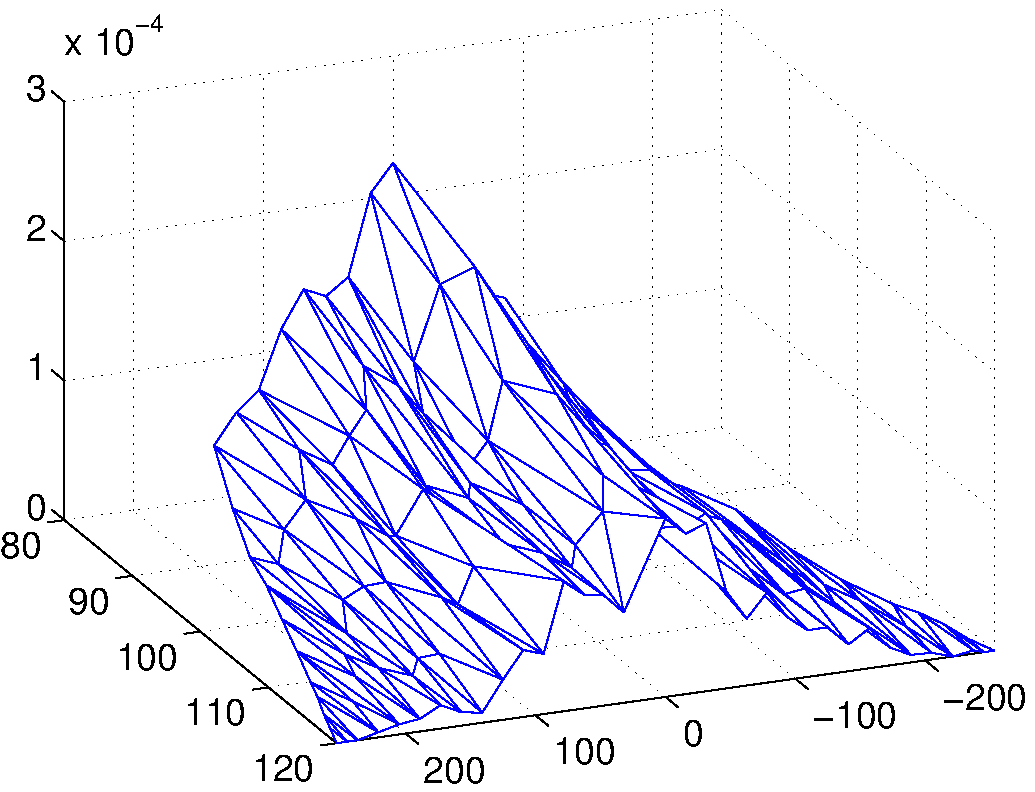
\includegraphics[width=\textwidth]{figures/hmm_pdf_sigma_1}
\end{center}
\caption{HMM solution for $\sigma = 1$. 2000 samples are used to produce this PDF.}
\end{figure}

\begin{figure}
\begin{center}
\includegraphics[width=\textwidth]{figures/hmm_pdf_sigma_1.5.eps}
\end{center}
\caption{HMM solution for $\sigma = 1.5$. 4000 samples are used to produce this PDF.}
\label{f:hmm sigma=1.5}
\end{figure}

It is worth mentioning that producing the solutions shown in Figures \ref{f:hmm sigma=.5} to \ref{f:hmm sigma=1.5} take several hours whereas the solutions produced with the FEM takes no more than a few minutes. Establishing exact figures on the computational advantage of FEM methods over SDE methods would require additional work; numerical parameters should be chosen optimally, and parallelized algorithms should be implemented. Nonetheless, the large difference in computation times between the two methods suggests that averaging methods can lead to significantly faster computational methods. It seems plausible that in some circumstances, problems that have been deemed too complicated could be solved if stochastic averaging methods were used.

%%% Local Variables: 
%%% mode: latex
%%% TeX-master: "main"
%%% End:
